% EOD Documentation Paper #3
% Project initiated Dec 22 2013

%\documentclass{emulateapj}
% Requirement of PASP to use preprint and aastex
\documentclass[11pt,preprint]{aastex}
\usepackage{amsmath,amssymb}
\usepackage{xspace}
\usepackage{graphicx}
\bibliographystyle{apj} 
\usepackage{epstopdf}  
\usepackage{graphicx}
\usepackage{epsfig}
\usepackage{verbatim}
\usepackage{morefloats} % somehow need this to have lots of figures
                        % and tables?
% for attractive links:
\usepackage[colorlinks,urlcolor=blue,citecolor=black,linkcolor=blue]{hyperref}
%\usepackage[nolists]{endfloat} % put floats at end - doesn't work
\interfootnotelinepenalty=10000 % Do not want cross-page footnote!

\usepackage{CJK} 

% definition of symbols
\def\beq{\begin{equation}}
\def\eeq{\end{equation}}
\def\ergcms{erg~cm$^{-2}$~s$^{-1}$}
\def\ergs{erg~s$^{-1}$}
\def\mps{m~s$^{-1}$}
\def\msun{M_{\odot}}
\def\lsun{L_{\odot}}
\def\etal{~et~al.~}
\def\degree{^{\circ}}
\def\leq{\leqslant}
\def\geq{\geqslant}
\def\micron{$\mu$m}
\def\percm2{{\rm cm^{-2}}}
\def\peryr{yr$^{-1}$}
\def\kepler{\textit{Kepler}}
\def\spitzer{\textit{Spitzer}}
\def\micron{$\mu$m}
\def\mjup{$M_{\rm Jup}$}
\def\rearth{R_\oplus}


\maxdeadcycles=1000 % need this to have bunch of figures on each page
                    % at end

\slugcomment{}
\shorttitle{}
\shortauthors{}

%%%%%%%%%%%%%%%%%%%%%%%%%%%%%%%%%%%%%%%%%%%%%%%%%%%%%%%%%%%%%%%%%%%%%%%%%%%%%%%%%%%%%%%%%%%%%%%%%%%%
\begin{document}

\begin{CJK*}{UTF8}{gbsn}

\title{The Exoplanet Orbit Database 2, 2014 updates}

% leading authors
\author{Eunkyu Han\altaffilmark{1,2}}
\author{Sharon X. Wang\altaffilmark{1,2,3}}
\author{Jason T. Wright\altaffilmark{1,2,3}}
\author{Ying Feng\altaffilmark{1,2}}
\author{Ming Zhao\altaffilmark{1,2}}
\author{Onsi Fakhouri}
\author{and Friends}

\altaffiltext{1}{Department of Astronomy \& Astrophysics, 525 Davey
  Lab, The Pennsylvania State University, University Park, PA 16802, USA;
  Send correspondence to datamaster@exoplanets.org.}
\altaffiltext{2}{Center for Exoplanets and Habitable Worlds, The
  Pennsylvania State University, University Park, PA 16802, USA}
\altaffiltext{3}{Astrobiology Research Center, The
  Pennsylvania State University, University Park, PA 16802, USA} 


%%%%%%%%%%%%%%%%%%%%%%%%%%%%%%%%%%%%%%%%%%%%%%%%%%%%%%%%%%%%%%%%%%%%%%%%%%%%%%%%%%%%%%%%%%%%%%%%%%%%
\begin{abstract}
Make sure to mention: data are available at exoplanets.org; KOIs are included.
ZZZ Also mention the number of confirmed planets? and maybe the scope of the EOD (what are in our database)
\end{abstract}  

%%%%%%%%%%%%%%%%%%%%%%%%%%%%%%%%%%%%%%%%%%%%%%%%%%%%%%%%%%%%%%%%%%%%%%%%%%%%%%%%%%%%%%%%%%%%%%%%%%%%
\section{Introduction}\label{sec:intro}

% Recent development in exoplanet discoveries
Since the launch of NASA's \kepler\ mission \citep{Borucki2010}, the
number of confirmed exoplanets has increased from about 300 to over
1490 as of March 2014 (exoplanets.org). \kepler\ contributed to a vast
majority of these new discoveries ($> 800$) while providing an
additional sample of over 3000 exoplanet candidates (\kepler\ Objects
of Interest, KOIs; e.g.~\citealt{Batalha2013}). The transit method has
surpassed the radial velocity (RV) method and become the most fruitful
mean for detecting exoplanets. Meanwhile, great promises lie within
the new and future exoplanet surveys and instruments with direct
imaging (e.g., the Gemini Planet Imager, GPI,
\citealt{Macintosh2014}) and microlensing (e.g., the Wide-Field
InfraRed Survey Telescope, WFIRST, \citealt{Green2012}), while the
fronts of RV and transit exoplanet searches keep expanding (e.g., the
MINiature Exoplanet RV Array, MINERVA, \citealt{Wright2014}; and the
Transiting Exoplanet Survey Satellit, TESS, \citealt{Ricker2010}).

% The business of tracking planet discoveries and EOD
This paper describes the continuing efforts since \cite{Butler2006}
and \cite{Wright2011} to maintain the Exoplanet Orbit Database (EOD)
and the Exoplanets Data Explorer (EDE) to keep track of the exoplanet
discoveries and to catalog their orbital parameters and host star
properties. There are also other entities devoted to this effort,
including the Extrasolar Planets Encyclopaedia\footnote{See
  \url{http://exoplanet.eu}.}  \citep{Schneider2011} and the NASA
Exoplanet Archive\footnote{See
  \url{http://exoplanetarchive.ipac.caltech.edu}.}
\citep{Akeson2013}. As described in \cite{Wright2011}, the EOD is
dedicated to cataloging all \emph{robustly-detected} exoplanets with
\emph{well-determined} orbital parameters published in
\emph{peer-reviewed} literature.

% data access and popularity
The EOD is hosted by exoplanets.org, which also hosts the EDE, an
interactive table with plotting tools including all the EOD exoplanets
as well as other confirmed exoplanets (and now also KOIs). The entire
dataset of exoplanets.org is available for download as a single {\tt
  .csv} file at the website's front page.\footnote{At
  \url{exoplanets.org/csv-files/exoplanets.csv}.} The EOD is widely
used in exoplanet researches (e.g., \citealt{Dawson2013},
\citealt{Howard2013}, \citealt{Kipping2013}, \citealt{Kane2014},
\citealt{Weiss2014}), and the website exoplanets.org is among the most
visited exoplanet databases, with over $47,000$ visitors in 2013
according to Google Analytics.

% updates on EOD and the website
Since \cite{Wright2011}, the EOD has expanded its scope: we now do
not require the host star of an exoplanet to be a normal star (e.g.,
exoplanets around pulsars are now included). It has also ingested more
parameters describing the exoplanet systems and their host stars, and some
parameters are revised or deleted. We describe the updates with the
EOD in Section~\ref{sec:update}. The EDE at exoplanets.org has also
expanded its scope and now includes the \kepler\ exoplanet candidates
(KOIs). We describe these changes in Section~\ref{sec:kepler}. The
website exoplanets.org has gone through major back-end changes since
\cite{Wright2011}, which is described in Section~\ref{sec:website}. We
summarize the updates and possible future improvements in
Section~\ref{sec:summary}. 


%------------------------------------------------------------------
% RECYCLE BIN
\begin{comment}
Since the first peer-reviewed list of exoplanets with robust orbits
\citep{Butler2002,Butler2006}, the count of exoplanets has increased
from less than 200 to over 1490 as of March 2014
(exoplanets.org). Before the launch of NASA's \kepler\ mission
\citep{Borucki2010}, most confirmed exoplanets were discovered via the
precise radial velocity (RV) method. However, since 2009, \kepler\ has
contributed over $\sim$ 800 confirmed exoplanets (e.g.,
\ciatealt{Marcy2014}, \citealt{Rowe2014}) as well as over 3000
exoplanet candidates (\kepler\ Objects of Interest, KOIs;
e.g.~\citealt{Batalha2013}).

As the number of exoplanet discoveries keeps rising, it is important
to keep track of these discoveries and cataloging the orbital
parameters and host star properties of exoplanet systems. There are
several entities that are devoted to this effort, including the
Exoplanet Orbit Database (EOD) and Exoplanets Data Explorer\footnote{See
  \url{http://exoplanets.org}.} \citep{Wright2011}, the Extrasolar
Planets Encyclopaedia\footnote{See \url{http://exoplanet.eu}.}
\citep{Schneider2011}, the NASA Exoplanet Archive\footnote{See
  \url{http://exoplanetarchive.ipac.caltech.edu}.}
\citep{Akeson2013}, and so on.

This paper describes the continuing efforts since \cite{Wright2011} to
maintain the EOD and the Exoplanets Data Explorer at exoplanets.org.

The efforts of keeping track of exoplanet discoveries are being
carried out by several entities, and most notably, the Extrasolar
Planets Encyclopaedia\footnote{See \url{http://exoplanet.eu}.}
\citep{Schneider2011}, the NASA Exoplanet Archive\footnote{See
  \url{http://exoplanetarchive.ipac.caltech.edu}.}
\citep{Akeson2013}, and the Exoplanet Orbit Database (EOD) and
Exoplanets Data Explorer\footnote{See \url{http://exoplanets.org}.}
\citep{Wright2011}.
\end{comment}
%------------------------------------------------------------------


%%%%%%%%%%%%%%%%%%%%%%%%%%%%%%%%%%%%%%%%%%%%%%%%%%%%%%%%%%%%%%%%%%%%%%%%%%%%%%%%%%%%%%%%%%
\section{Updates on the EOD}\label{sec:update}

The scope of the EOD has expanded, and there are two major changes
from what was described in \cite{Wright2011}. Previously, we only
included exoplanets orbiting the ``normal stars", but now we are not
limiting the type of host stars (e.g. we included exoplanets orbiting
neutron stars). Furthermore, in \cite{Wright2011}, we only had
exoplanets that were discovered by the RV and transit methods in the
EOD, but now we also have planets discovered via timing. For the
future, exoplanets discovered by any other methods with robust
detections and good orbital parameters will also be included in the
EOD.

The rest of the selection criteria for the EOD remain unchanged. We
still require the planets to be smaller than 24 \mjup\ and to have
robust detections and well-determined orbits (though these are not
strictly quantitative; see Section~2 of \citealt{Wright2011}). When
new evidence comes to light and we are no longer confident about the
planet, we remove it from EOD, even if the evidence is not peer
reviewed. 

The purpose of the EOD has not changed: we aim to provide the readers
with a comprehensive, reliable, and up-to-date database of exoplanets
with good orbital parameters and host star properties. We do not
report \textit{all} the announced exoplanets as we are not trying to
do ``an encyclopedic presentation of every claimed detection of an
exoplanet" \citep{Wright2011}.

In the following subsections, we describe the newly added and revised
fields since \cite{Wright2011}, but list all fields in
Table~\ref{tab:par}. We divide the fields into categories in
consistency with the individual planet page on
exoplanets.org. Figure~\ref{fig:individual} is an example of
individual planet page. Some fields are not explicitly tabulated on
the page (e.g., the URLs), but are explicitly listed in the
downloadable {\tt .csv} file (see Section~\ref{sec:intro}). Though we
focus on the EOD in this section, the fields apply to all planets on
exoplanets.org. We follow the definition of orbital elements in
\cite{Wright2013} unless indicated otherwise.


%------------------------------------------------------------------------------
\subsection{Discovery and References}\label{sec:disc}

We report general information of when, by whom and how the planets
were discovered and provide the references. We describe the added or
revised fields since \cite{Wright2011} below.

{\bf DISCMETH} field previously reported the method of discovery,
which was either radial velocity or transit. We have replaced DISCMETH
with {\bf PLANETDISCMETH} and \mbox{{\bf STARDISCMETH}} to better
report how exoplanet systems and individual exoplanets are first
discovered. PLANETDISCMETH reports the discovery method for the
planet, wihle STARDISCMETH reports the discovery method for the first
discovered planet around the host star. Furthermore, they are stored
in string formats and have values of one of the following: RV,
Transit, Imaging, Microlensing, Timing, or Astrometry.

{\bf MONTH} field reports the month in integer of when the
peer-reviewed paper is accepted by the journal.

{\bf KEPID} stands for KEPler ID, which is the integer number assigned
for a Kepler host star. KEPID is only available for the unconfirmed
KOI which we import directly from the Exoplanet Archive. Therefore,
none of the EOD planets and the confirmed Kepler planets has KEPID.

{\bf KOI} stands for Kepler Objects of Interest, which is an object
with transit signals detected by \kepler\ but have not been confirmed
to be due to exoplanets. The KOI field contains a floating point
number that consist of a whole number designated to the host star
followed by a decimal number denoting a candidate planet. For example,
KOI 102 is a star suspected to host two exoplanets, and KOI 102.01 is
the inner planet candidate and KOI 102.02 is the outer one. Once a
candidate is confirmed, the NAME field of the planet is replaced by
the official \kepler\ ID (``Kepler" followed by a hyphen, an integer
and an lower case letter). The KOI number is then used as
OTHERNAME. None of the KOIs are in the EOD. For more information, see
Section~\ref{sec:kepler}.

{\bf EOD} is a flag which indicates whether an exoplanet is included
in the EOD for having robust detection and well-characterized orbital
parameters such as the orbital period (PER). EOD equals 1 means the
exoplanet is in the EOD. We added this field because exoplanets.org
now also includes robustly discovered planets that do not have
well-characterized orbits, and also \kepler\ planet candidates (see
Section~\ref{sec:kepler} for more details).

{\bf MICROLENSING, IMAGING, TIMING and ASTROMETRY} are flags which
indicate that a planet detected via theses methods. For example,
MICROLENSING $=$ 1 means the planet is detected in a microlensing
event. However, we require the detection to be robust, as determined
by the QUAlity Control Board of the Exoplanet Database, QUACBED (see
Section~\ref{sec:kepler}). 


%------------------------------------------------------------------------------
\subsection{Orbital Parameters}\label{sec:orbit}

We report the orbital parameters that determine the shape of the
planet's orbit. Depending on the detection methods, different sets of
parameters are given by the literatures. For instance, if a planet is
detected by the radial velocity method, the semiamplitude, $K$, is
reported whereas the inclination of the orbit, $i$, is reported by the
transit method. We describe the added fields since \cite{Wright2011}
below.  

{\bf MASS} is the mass of the planet in the unit of Jupiter
mass. Previously, we only reported the minimum mass, ($m\sin{i}$,
MSINI) of the planets. We now report the mass as well when it is
available. For example, if a planet is discovered by microlensing, we
report the actual mass of the planet according to the literature. If a
planet has both radial velocity and transit measurements, we calculate
the mass from the minimum mass $m\sin{i}$ and the orbital inclination
$i$. MASS is set to MSINI if the orbital inclination is not given and
the reference for MASS, MASSREF is set to ``Set to MSINI; I unknown''.

For KOIs without MSINI measured, we calculate their mass using the
mass-radius relation from the literatures. For KOIs with $R<4\rearth$,
we follow \cite{Weiss2014}; for $4\rearth<R<6\rearth$, we follow
\cite{Lissauer2011}; and for $6\rearth<R<11.7\rearth$ we follow
\cite{Mordasini2012}.  

{\bf SEP} is the projected separation on the sky between the host star
and the planet in the unit of AU. For directly imaged planets, the
literatures usually report the projected separation and we report the
value accordingly.  If SEP is not directly measured but the semi-major
axis ($a$, A) is available, then SEP is set to A with its reference,
SEPREF, set to ``Set to A''. For the cases where only the projected
separation is given but A is not available (e.g., the directly imaged
planets), then A is set to SEP.

{\bf I} is the orbital inclination. Previously, only transiting
systems have I measured, but now some non-transiting systems
have I's reported too. For example, one microlensing system,
OGLE-2006-BLG-109L, has I measured \citep{Bennett2010}.

{\bf BIGOM} is the longitude of the ascending node ($\Omega$) in the
unit of degree. At the moment, this is only measured for some of the
directly imaged planets, which are not in the EOD.

{\bf LAMBDA} is the projected spin-orbit misalignment ($\lambda$) in
the plane of the sky in the unit of degree. At the moment, $\lambda$
values are only available for the transiting systems, which are
measured by either the Rossiter-McLaughlin effect
\citep[e.g.,][]{Winn2005} or planet transiting star spots
\citep[e.g.,][]{Sanchis-Ojeda2012}. $\lambda$ is introduced because
the true spin-orbit angle ($\phi$), defined as the angle between the
stellar spin axis and the orbital axis, is normally not directly
measurable. We follow the definition of $\lambda$ in
\cite{Fabrycky2009} where the coordinates are defined as follows: the
$z$-axis points toward the observer, the $x$-axis points along the
intersection of the sky plane and the planet's orbital plane with the
ascending node of the planet having $x<0$, and the $y$-axis completes
a right handed-triad. $\lambda$ is measured clockwise on the sky from
the $y$-axis to the projected stellar rotational axis. $\lambda$ is
not a newly added field but we describe it here because it was not
reported consistently since some literatures report the ``projected
spin-orbit misalignment" as $\beta = -\lambda$ instead. We have sorted
these cases out and made sure that our $\lambda$'s are following the
definition of \cite{Fabrycky2009}.

{\bf MASSREF} and {\bf MASSURL} fields were used to report the
reference and the URL of stellar mass but now they are used for planet
mass.

%------------------------------------------------------------------------------
\subsection{Transit Parameters}\label{sec:transit}

We report the transit parameters, which are available only when the
planet has TRANSIT flag equal to 1. We describe added fields since
\cite{Wright2011} below.

{\bf DR} is the distance between the planet and the star during the
transit in stellar radii. This is one of the parameters that goes into
the transit light curve modeling (see e.g. \citealt{Batalha2013}).

{\bf RR} is the ratio of the planetary radius and the stellar
radius. If the transit depth (DEPTH) is not given, we calculate DEPTH
by taking square of RR but we do not calculate RR from DEPTH.


%------------------------------------------------------------------------------
\subsection{Secondary Eclipse}\label{sec:se}

We have added an entirely new set of fields for the secondary
eclipse. Previously, due to the limits of instrumentation, there were
not much available measured secondary eclipse depths. Since
\cite{Wright2011}, as many different surveys have been launched,
secondary eclipse depths at multiple bands are now
available. Therefore, we added this entire new set of fields since.

{\bf SE} flag indicates whether the system has detected secondary
eclipse in any of the two Micron All-Sky Survey (2MASS;
\citealt{Skrustskie2006}) $J$, $H$, and $K_s$, Kepler photometry band,
and 4 Spitzer IRAC bands. SE is a boolean and being true indicates the
system has at least one detected secondary eclipse.

{\bf SEDEPTHX} whereas X stands for one of J H KS KP 36 45 58 80:
these fields are the secondary eclipse depth measured in the
corresponding wavelength band. SEDEPTHJ, H, and KS are the depths
measured in the 2MASS wavelength band in near infrared each centered
at 1.25~\micron, 1.65~\micron, and 2.15~\micron, respectively. KP is
the depth measured in the \kepler\ photometry band which ranges from
400 to 865~nm. The rest four stand for the Spitzer bands centered at
3.6~\micron, 4.5~\micron, 5.8~\micron, and 8.0~\micron.

{\bf SET} is the epoch of secondary eclipse center in HJD.

%------------------------------------------------------------------------------
\subsection{Stellar Properties}\label{sec:stellarprop}

This set of parameters is to provide users the physical parameters of
the exoplanet host stars.  Most of the parameters are derived from the
stellar models in the literatures and we provide the readers with the
references. We describe added fields since \cite{Wright2011} below.

{\bf GAMMA} ($\gamma$) is the radial velocity of the center of mass of
the planetary system and is reported in km/s.

{\bf RSTAR} is the radius of the star in the solar radius.

{\bf RHOSTAR} is the density of the star in the unit of g/cm$^3$.

%------------------------------------------------------------------------------
\subsection{Stellar Magnitudes}\label{sec:stellarmag}

We provide the brightness of the host star measured in different
wavelengths. We report optical magnitudes ($V$ and $B-V$), 2MASS $J$,
$H$, and $K_s$ magnitudes and we added {\bf KP} since
\cite{Wright2011}, which is the stellar magnitude measured through the
Kepler bandpass.


%------------------------------------------------------------------------------
\subsection{Coordinates and Catalogs}\label{sec:coord}
We report the coordinates of the host star as well as the stellar ID
as designated by different catalogs.  We added {\bf DIST} since
\cite{Wright2011}, which is the distance of the host star in the unit
of pc. If only parallax (PAR) is given, we convert it to DIST and vice
versa. If the literature does not report DIST or PAR, then we obtain
PAR from the Hipparcos data set by \cite{van Leeuwen2009}.

We naively propagate the error in PAR to DIST. 

%------------------------------------------------------------------------------
\subsection{Uncertainties and Upper Limits}\label{sec:unc}

We now report uncertainties for a certain field X as XUPPER, XLOWER
and UX. XUPPER and XLOWER store the upper and lower 1$\sigma$
uncertainties, and they are different when the error bars are
asymmetric. UX contains the 1$\sigma$ uncertainty, and it equals to
$({\rm XUPPER+XLOWER})/2$ in the case of asymmetric error bars. Fields
that have XUPPER, XLOWER and UX are: all the orbital parameters except
for TREND and FREEZE\_ECC flags; all the transit parameters except for
TRANSIT flags; all the secondary eclipse fields except for SE flag;
and all the stellar properties except for STAR, SPECREF and BINARY
flag; and DIST and PAR.

We also report the upper limits (XUL) for planet mass (MSINI),
eccentricity (ECC), and the velocity semi-amplitude (K) when the
literatures report them. For example, the upper limits for ECC is
reported when the orbit is circular, and the upper limits for K is
reported when there is no radial velocity detection. If only upper
limits are given, we set the field to 0, the uncertainty to half of
the upper limit, and the upper limits to the upper limits. For
example, if the literature reports the upper limit for ECC, then we
put the value in ECCUL, set ECC to be 0, ECCUPPER to ECCUL, and UECC
to ECCUL/2. Since not all authors define the upper limits in the same
way (e.g. 1$\sigma$ or some fixed percentile), we encourage the
readers to refer to the literature for more information.

%------------------------------------------------------------------------------
\subsection{References}\label{sec:ref}

The fields {\bf XREF} and {\bf XURL} store the peer-reviewed reference
and link to the publication for the field X.

Previously, we only reported general references (e.g. FIRSTREF,
FIRSTURL, ORBREF, and ORBURL), but now we report the references for
most of the fields.

RA, DEC, and PAR do not have references but they are from the
\textit{Hipparcos} by \cite{van Leeuwen2009}. $B-V$ (BMV) field does
not have a reference but the values are from the \textit{Hipparcos}
catalog by \cite{Perryman1997}. The fields J H and KS do not have
references as well but they are from the 2MASS
\citep{Skrutskie2006}. The KP field do not have reference but the
values are from the Exoplanet Archive \citep{Akeson2013}.

SHK and RHK are poorly maintained fields and they unreferenced at the
moment though we plan to include proper reference in the future. Most
of the values are from \cite{Butler2006}.

%------------------------------------------------------------------------------
\subsection{Removed Fields}\label{sec:removed}

We removed 2 fields. 

{\bf SPSTAR} field previously reported the stellar type of the host
star but it is removed since it is not reliable. 

{\bf NSTEDID} field reported ID of host star in NStED and now it is
replaced by EANAME, which is the name of the star as appears on the
NASA's Exoplanet Archive \citep{Akeson2013}. 


%------------------------------------------------------------------------------
% Figure: single planet page
\begin{figure}[!htb]
\centering

\includegraphics[width=\textwidth]{../fig/wasp-14b.eps}
\caption{An example page for an individual exoplanet (WASP-14b in this
  case). The numbers listed in each field contain links to the
  reference on NASA ADS. In this example for WASP-14b, we provide the plot
  for the phased RVs, but we are yet to implement such feature for all
  planets with available RV data.}
\label{fig:individual}
\end{figure}


%%%%%%%%%%%%%%%%%%%%%%%%%%%%%%%%%%%%%%%%%%%%%%%%%%%%%%%%%%%%%%%%%%%%%%%%%%%%%%%%%%%%%%%%%%%
\section{Inclusion of the Kepler Planet Candidates and Other Exoplanets on Exoplanets.org}\label{sec:kepler}

Since \cite{Wright2011}, as more planets were robustly discovered by
different methods other than radial velocity and transit, we have
expanded our database at exoplanets.org to better ingest those
planets.

% KOIs
First, we now include the KOIs discovered by \kepler\ in the
EDE. Although KOIs are not counted as part of the EOD due to their
status of being ``candidates", we include them in our website so that
these KOIs are put into the context of all confirmed exoplanets. The
KOIs listed in our table include three Kepler data releases (as of
March 2014), and we always keep up with the most up-to-date
releases. The original data are from the NASA Exoplanet Archive.

To display the KOIs in the EDE table, check the ``Kepler" option on
the upper left of the table (default selection only includes ``Orbit
Database", i.e.~the EOD, and ``Other"). They can also be displayed on
plots with the interactive plotting tool of EDE (see
Figure~\ref{fig:koi} for an example plot).

% Other Planets
Second, we now also include
robustly detected imaging, microlensing, and timing planets, and our
criteria for a `robust detection' are the following (as set by the
QUACBED):

\begin{itemize}
\item Imaging planets:
\begin{enumerate}
\item Planet-star mass ratio $q < 0.024$ ($< 24\ $\mjup\ for a solar
  mass star); and in general we require ($q+\sigma_q$) $< 0.024$,
  where $\sigma_q$ is the uncertainty in $q$.
\item SEP $<$ 100 AU $\times$ ($M_*/M_\odot$), where SEP is the
  semi-major axis a if a is known, and the projected separation
  otherwise.
\item Confidently detected: the detection is clearly of a real
  astrophysical source, and will unlikely later be found to have been
  spurious.
\item Confidently bound: in opinion of the QUACBED the object will not
  be later found to be unbound or a chance alignment.

\end{enumerate}
\item Microlensing planets:\\
We accept microlensing planets that appear in refereed journals as
having unambiguously planetary masses (planet host mass ratio,
$q<0.024$). In cases of ambiguity, we consult with QUACBED.  

\item Timing planets:\\
 Timing planets must have dynamically stable orbits and, ideally, show
 multiple complete orbits (e.g., see \citealt{Wittenmyer2012},
 \citealt{Horner2012}, and \citealt{Wittenmyer2013}). 

\end{itemize}
Some of the exoplanets primarily detected by these methods do not have
well-determined orbital parameters, and thus they are categorized as
``Other Planets'' on exoplanets.org instead of being in the EOD. These
planets can be displayed by check the `Other' option for the EDE
table. As of March 2014, no microlensing or imaging planets are in the
EOD, while several timing exoplanets have well-determined orbital
parameters and are included in the EOD. Moreover, there have been no astrometry planets in the EOD but we plan to include them if any robust detections occur.


%------------------------------------------------------------------------------
% Figure: single planet page
\begin{figure}[!htb]
\centering
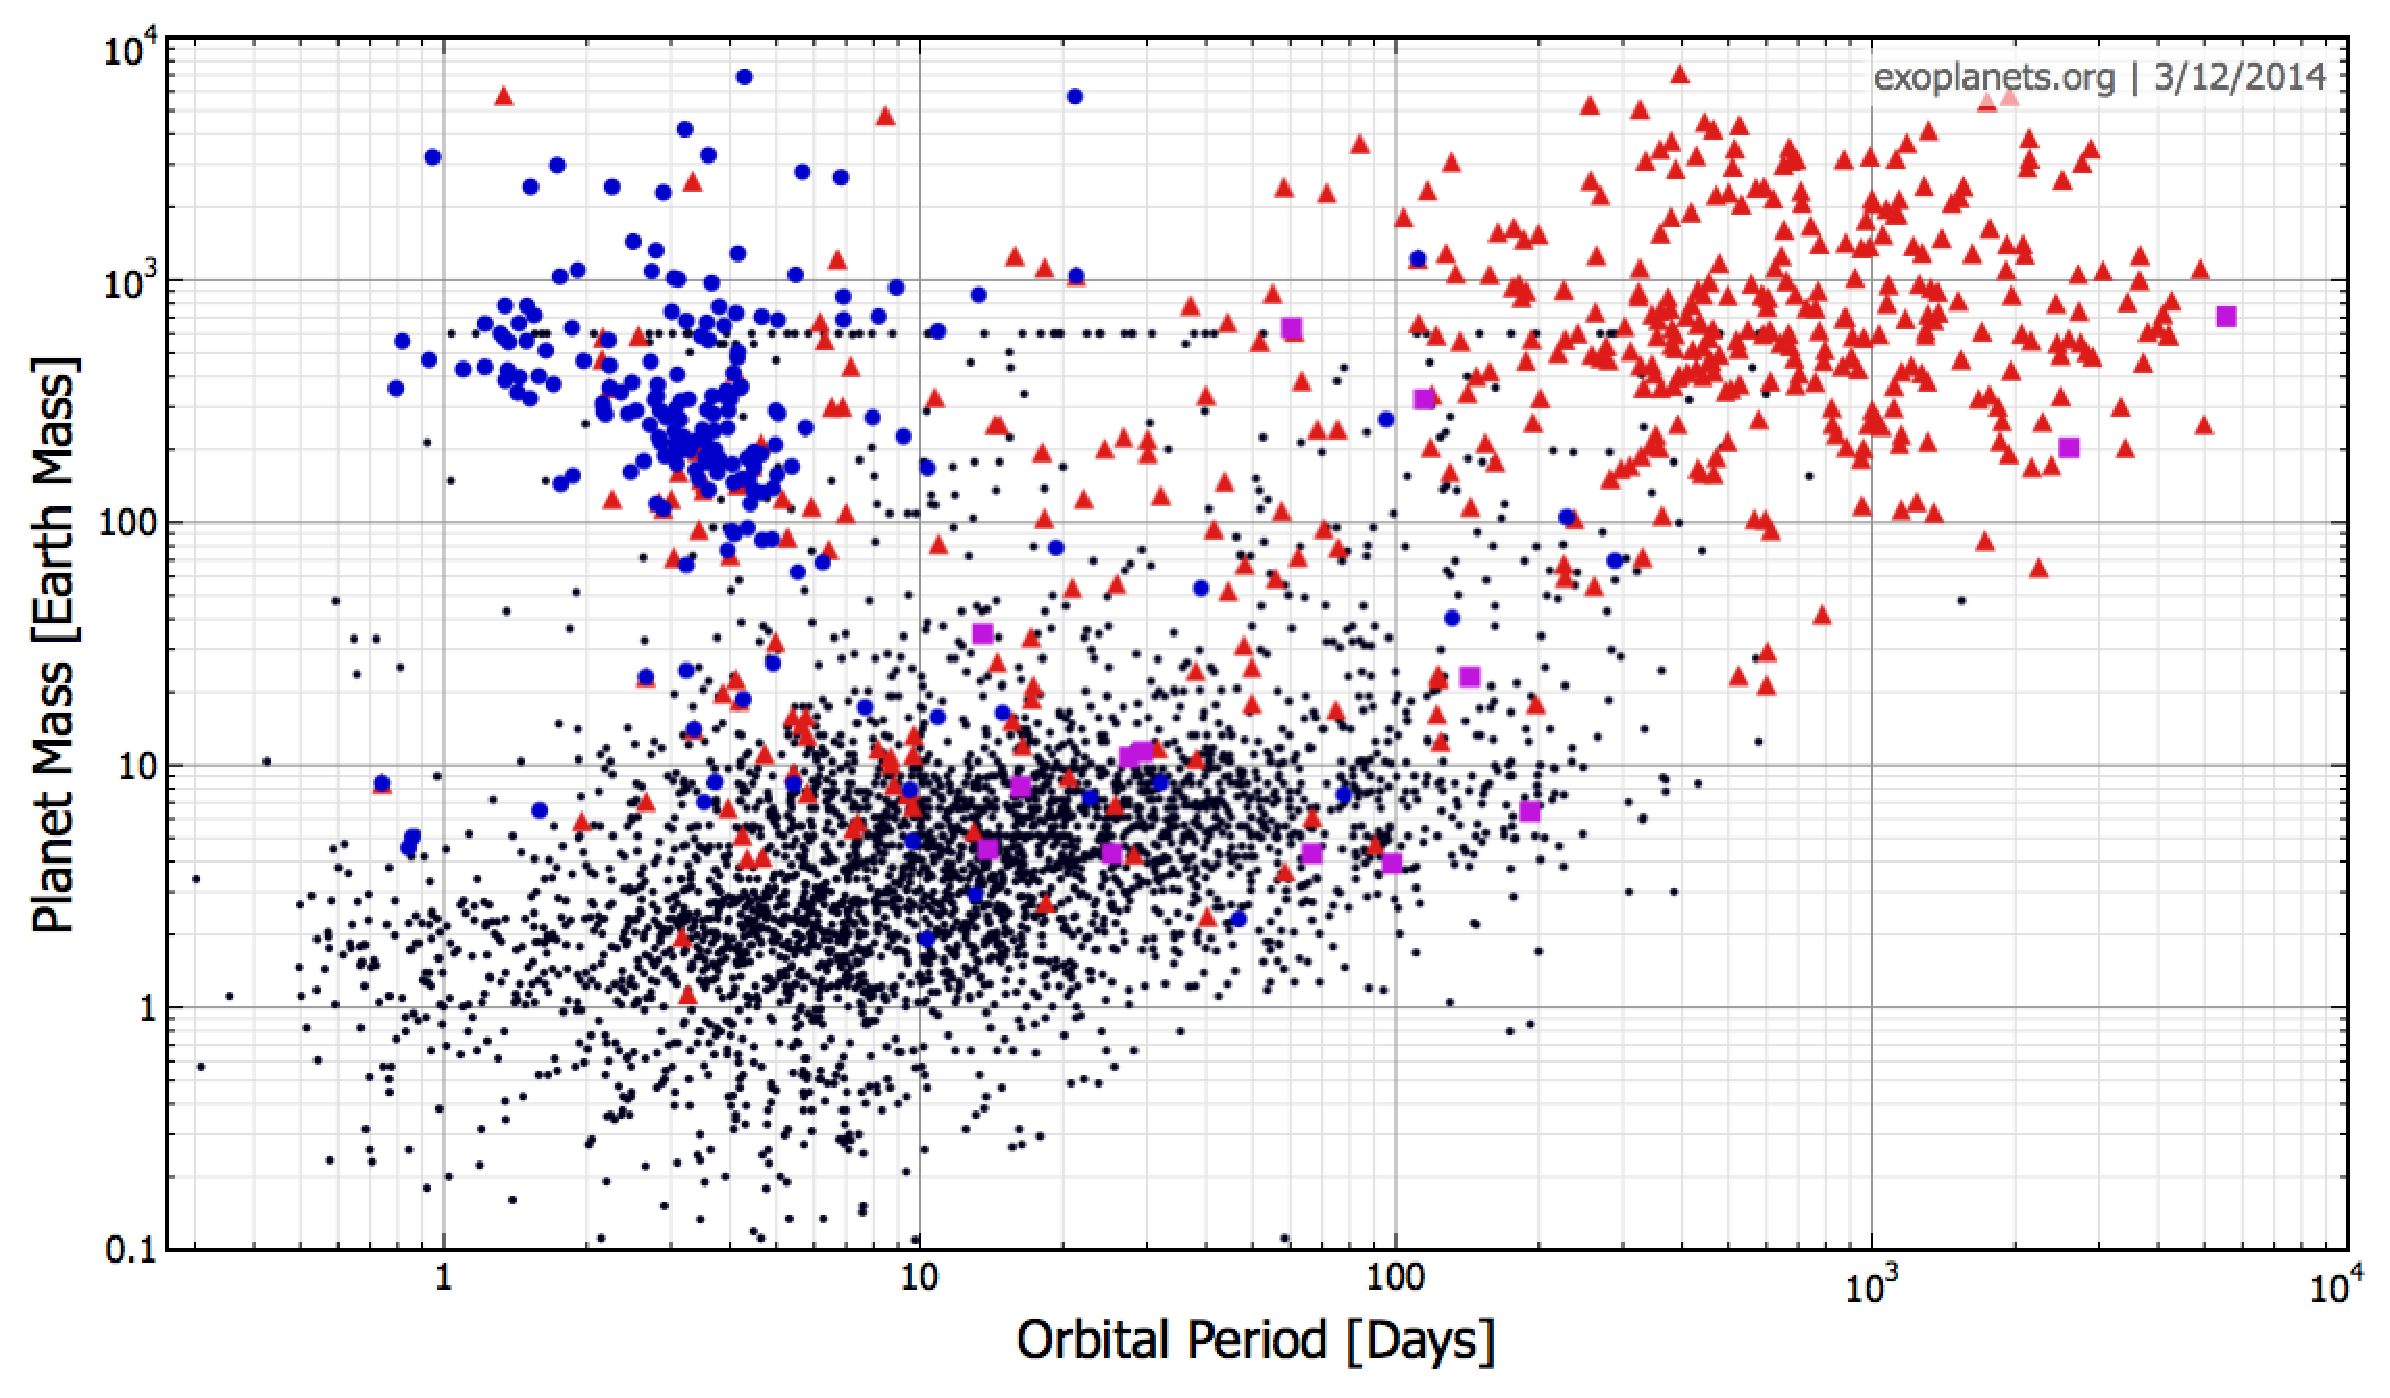
\includegraphics[width=\textwidth]{../fig/mass-per-color.eps}
\caption{An example plot produced by the interactive plotting tools of
  EDE on exoplanets.org. The $x$-axis is planet orbital period in days
  and $y$-axis is planet mass in Earth's mass. The exoplanet samples
  being plotted are the ones in the EOD, including transit planets
  (blue large dots), RV planets (red triangles), and timing planets
  (magenta squares). The KOIs are plotted as black small dots, and
  their masses are calculated using their radii based on mass-radius
  relations from the literature (see Section~\ref{sec:orbit}).}
\label{fig:koi}
\end{figure}


%%%%%%%%%%%%%%%%%%%%%%%%%%%%%%%%%%%%%%%%%%%%%%%%%%%%%%%%%%%%%%%%%%%%%%%%%%%%%%%%%%%%%%%%%%%
\section{Updates on the Website}\label{sec:website}

Onsi? Essential updates on the website.


%%%%%%%%%%%%%%%%%%%%%%%%%%%%%%%%%%%%%%%%%%%%%%%%%%%%%%%%%%%%%%%%%%%%%%%%%%%%%%%%%%%%%%%%%%%
\section{Summary and Future Work}\label{sec:summary}

We have had two major updates since \cite{Wright2011}. First, we
changed the scope of the EOD. We removed the limit on the type of the
host star. We included the planets discovered by various methods
(e.g. timing) in the EOD. We also have added some new fields, removed
obsolete fields and revised them as necessary.

Second, we included Kepler planet candidates and other planets on
exoplanets.org. Although they are not included in the EOD, we reported
them on our website to help the users explore them and use them
easily.

ZZZ add summary for Onsi's section.


We hope to include images of directly imaged planets (where allowed under copyright law) and
light curves for transits in the future.


%%%%%%%%%%%%%%%%%%%%%%%%%%%%%%%%%%%%%%%%%%%%%%%%%%%%%%%%%%%%%%%%%%%%%%%%%%%%%%%%%%%%%%%%%%%
\acknowledgments

NSF funding?

SXW acknowledges support from PSARC. This research has made use of
NASA's Astrophysics Data System Bibliographic Services (ADS). 


%%%%%%%%%%%%%%%%%%%%%%%%%%%%%%%%%%%%%%%%%%%%%%%%%%%%%%%%%%%%%%%%%%%%%%%%%%%%%%%%%%%%%%%%%%%
% References:
%\newpage
% List references here
\begin{thebibliography}

\bibitem[Akeson et al.(2013)]{Akeson2013} Akeson, R.~L., et al.\ 2013, 
\pasp, 125, 989 % NASA Exoplanet Archive

\bibitem[Batalha et al.(2013)]{Batalha2013} Batalha, N.~M., et al.\ 2013, 
\apjs, 204, 24 % example of KOI release

\bibitem[Bennett et al.(2010)]{Bennett2010} Bennett, D.~P., et al.\ 2010, 
\apj, 713, 837 % OGLE microlensing planet with inclination measured

\bibitem[Borucki et al.(2010)]{Borucki2010} Borucki, W.~J., et al.\ 2010, 
Science, 327, 977 % Kepler instroduction and first results

\bibitem[Butler et al.(2002)]{Butler2002} Butler, R.~P., et al.\ 2002, 
\apj, 578, 565 % first peer-reviewed list of planets with robust orbits

\bibitem[Butler et al.(2006)]{Butler2006} Butler, R.~P., et al.\ 2006, 
\apj, 646, 505 % EOD first paper

\bibitem[Chauvin et al.(2012)]{Chauvin2012} Chauvin, G., et al.\ 2012, 
\aap, 542, A41 % beta Pic orbital pars

\bibitem[Collier Cameron et al.(2010)]{Collier Cameron2010} Collier 
Cameron, A., et al.\ 2010, \mnras, 407, 507 % WASP-33b having no RV
                                % detection and K upper limit

\bibitem[Cosentino et al.(2012)]{Cosentino2012} Cosentino, R., et al.\ 
2012, \procspie, 8446, 1V % HARPS-North

\bibitem[Dawson \& Murray-Clay(2013)]{Dawson2013} Dawson, R.~I., \&
  Murray-Clay, R.~A.\ 2013, \apjl, 767, L24  % use of EOD

\bibitem[Fabrycky \& Winn(2009)]{Fabrycky2009} Fabrycky, D.~C., \&
  Winn, J.~N.\ 2009, \apj, 696, 1230 % spin-orbit misalignment lambda definition
  
\bibitem[Green et al.(2012)]{Green2012} Green, J., et al.\ 2012, 
arXiv:1208.4012   % WFIRST

\bibitem[Horner et al.(2012)]{Horner2012} Horner, J., Wittenmyer, R.~A., 
Hinse, T.~C., \& Tinney, C.~G.\ 2012, \mnras, 425, 749 % dynamic
                                % analysis on timing planet

\bibitem[Howard(2013)]{Howard2013} Howard, A.~W.\ 2013, Science, 340,
  572 % use of EOD

\bibitem[Johnson et al.(2011)]{Johnson2011} Johnson, J.~A., et al.\ 2011, 
\apjs, 197, 26 % HD 116029B having ECC upper limit (circular orbit)
  
\bibitem[Kane(2014)]{Kane2014} Kane, S.~R.\ 2014, \apj, 782, 111 % use
                                % of EOD
  
\bibitem[Kipping(2013)]{Kipping2013} Kipping, D.~M.\ 2013, \mnras,
  434, L51 % use of EOD

\bibitem[Lagrange et al.(2009)]{Lagrange2009} Lagrange, A.-M., Gratadour, D., Chauvin, G., et al.\ 2009, \aap, 493, L21 %beta Pic b, imaging planet with I measured

\bibitem[Lissauer et al.(2011)]{Lissauer2011} Lissauer, J.~J., et al.\ 
2011, \apjs, 197, 8 % Mass-Radius for 1 Re < R < 6 Re

\bibitem[Macintosh et al.(2014)]{Macintosh2014} Macintosh, B., Gemini 
Planet Imager instrument team, Planet Imager Exoplanet Survey, G., 
\& Observatory, G.\ 2014, American Astronomical Society Meeting
Abstracts, 223, \#229.02  % GPI

\bibitem[Marcy et al.(2014)]{Marcy2014} Marcy, G.~W., et al.\ 2014, \apjs, 
210, 20 % 42 RV confirmed small Kepler planets

\bibitem[Mahadevan et al.(2012)]{Mahadevan2012} Mahadevan, S., 
Ramsey, L., Bender, C., et al.\ 2012, \procspie, 8446, %HPF  

\bibitem[Mordasini et al.(2012)]{Mordasini2012} Mordasini, C., Alibert, Y., 
Georgy, C., Dittkrist, K.-M., Klahr, H., \& Henning, T.\ 2012, \aap, 547, A112
% Mass-Radius for 6 Re < R < 11.684 Re

\bibitem[Moutou et al.(2011)]{Moutou2011} Moutou, C., D{\'{\i}}az, R.~F., Udry, S., et al.\ 2011, \aap, 533, A113  %Lambda example

\bibitem[Nielsen et al.(2014)]{Nielsen2014} Nielsen, E.~L., et al.\ 2014, 
arXiv:1403.7195 % beta Pic orbit pars
  
\bibitem[Perryman \& ESA(1997)]{Perryman1997} Perryman, M.~A.~C., \&
  ESA 1997, ESA Special Publication, 1200 % Hipparcos B-V reference

\bibitem[Ricker(2014)]{Ricker2014} Ricker, G.~R.\ 2014, Journal of the 
American Association of Variable Star Observers (JAAVSO), 42, 234 % TESS

\bibitem[Rowe et al.(2014)]{Rowe2014} Rowe, J.~F., et al.\ 2014, 
arXiv:1402.6534 % 715 new Kepler planets (multis)

\bibitem[Sanchis-Ojeda et al.(2012)]{Sanchis-Ojeda2012} Sanchis-Ojeda, R., 
et al.\ 2012, \nat, 487, 449 % Kepler 30 system lambda measurement
                             % with star spot transit

\bibitem[Schneider et al.(2011)]{Schneider2011} Schneider, J., Dedieu, C., 
Le Sidaner, P., Savalle, R., \& Zolotukhin, I.\ 2011, \aap, 532, A79
% exoplanet.eu

\bibitem[Skrutskie et al.(2006)]{Skrutskie2006} Skrutskie, M.~F., et al.\ 
2006, \aj, 131, 1163 % 2MASS

\bibitem[Sotin et al.(2007)]{Sotin2007} Sotin, C., Grasset, O., 
\& Mocquet, A.\ 2007, \icarus, 191, 337 % Mass-Radius for M<1Me, R<1Re

\bibitem[van Leeuwen(2009)]{van Leeuwen2009} van Leeuwen, F.\ 2009, \aap, 
497, 209 % Hipparcos catalog

\bibitem[Weiss \& Marcy(2014)]{Weiss2014} Weiss, L.~M., \& Marcy,
  G.~W.\ 2014, \apjl, 783, L6  % Mass-Radius for R < 4Re to be implemented

\bibitem[Winn et al.(2005)]{Winn2005} Winn, J.~N., et al.\ 2005, \apj, 631, 
1215 % HD 209458b, the first Rossiter-McLaughlin lambda measurement

\bibitem[Wittenmyer et al.(2012)]{Wittenmyer2012} Wittenmyer, R.~A., 
Horner, J., Marshall, J.~P., Butters, O.~W., 
\& Tinney, C.~G.\ 2012, \mnras, 419, 3258 % dynamic analysis on timing
                                % planets

\bibitem[Wittenmyer et al.(2013)]{Wittenmyer2013} Wittenmyer, R.~A., 
Horner, J., \& Marshall, J.~P.\ 2013, \mnras, 431, 2150 % dynamic
                                % analysis on timing planets

\bibitem[Wright et al.(2011)]{Wright2011} Wright, J.~T., et al.\ 2011,
  \pasp, 123, 412 % EOD 2011 paper

\bibitem[Wright \& Gaudi(2013)]{Wright2013} Wright, J.~T., \& Gaudi, B.~S.\ 2013,
  Planets, Stars and Stellar Systems.~Volume 3: Solar and Stellar
  Planetary Systems, 489 % Review article with definition of orbital elements

\bibitem[Wright et al.(2014)]{Wright2014} Wright, J., et al.\ 2014, 
American Astronomical Society Meeting Abstracts, 223, \#148.31

\end{thebibliography}



%%%%%%%%%%%%%%%%%%%%%%%%%%%%%%%%%%%%%%%%%%%%%%%%%%%%%%%%%%%%%%%%%%%%%%%%%%%%%%%%%%%%%%%%%%%
% Table
\clearpage

% NEW ORGANIZATION ACCORDING TO INDIVIDUAL PLANET PAGE
\begin{deluxetable}{llllc}
  \center
\tabletypesize{\scriptsize}
%\rotate
\tablewidth{0pt}
\tablecaption{Fields of Exoplanet Orbit Database\label{tab:par}}
\tablehead{
  \colhead{Field} & \colhead{Data Type} & \colhead{Meaning} &
  \colhead{Related Fields\tablenotemark{a}} & \colhead{Ref.\tablenotemark{b}}
}
\startdata
%
\sidehead{\textbf{Discovery and References}}
NAME\dotfill & String & Name of planet & \nodata & W11 \\
OTHERNAME\dotfill & String & Other commonly used name of star & \nodata & \ref{sec:disc} \\
DATE\dotfill & Integer & Year of publication of FIRSTREF & \nodata & W11 \\
MONTH\dotfill & Integer & Month of publication of FIRSTREF & \nodata & \ref{sec:disc} \\
PLANETDISCMETH\dotfill & String & Method of discovery of planet & \nodata & \ref{sec:disc} \\
STARDISCMETH\dotfill & String & Method of discovery of first planet in system & \nodata & \ref{sec:disc} \\
ORBREF\dotfill & String & Peer-reviewed origin of orbital parameters & ORBURL & W11 \\
FIRSTREF\dotfill & String & First peer-reviewed publication of
planetary orbit & FIRSTURL & W11 \\
JSNAME\dotfill & String & Name of host star used in the Extrasolar
Planets Encyclopaedia & EPEURL & W11 \\
ETDNAME\dotfill & String & Name of planet used in the Exoplanet
Transit Database & ETDURL & W11 \\
EANAME\dotfill & String & Name of planet used in the Exoplanet
Archive database & EAURL & \ref{sec:removed} \\
SIMBADNAME\dotfill & String & Valid SIMBAD name of host star (or
planet, if available) & SIMBADURL & W11 \\
KEPID\dotfill & Long Integer & The unique \kepler\ star identifier &
\nodata & \ref{sec:disc} \\
KOI\dotfill & Float & KOI object number & \nodata & \ref{sec:disc} \\
%KDE\dotfill & Boolean & If true, planet appears in the \kepler\ archive & \nodata & \ref{sec:disc} \\
EOD\dotfill & Boolean & If true, planet is included in the EOD & \nodata & \ref{sec:disc} \\
MICROLENSING\dotfill & Boolean & If true, planet was detected via microlensing & \nodata & \ref{sec:disc} \\
IMAGING\dotfill & Boolean & If true, planet was detected via imaging & \nodata & \ref{sec:disc} \\
TIMING\dotfill & Boolean & If true, planet was detected via timing & \nodata & \ref{sec:disc} \\
ASTROMETRY\dotfill & Boolean & If true, planet was detected via astrometric motion & \nodata & \ref{sec:disc} \\
%
\sidehead{\textbf{Orbital Parameters}}
MSINI\dotfill & Float & Minimum mass (as calculated from the mass
function) in \mjup & -UL, -UPPER, etc. & W11 \\
MASS\dotfill & Float & Mass of planet in \mjup & -UPPER, etc. & \ref{sec:orbit} \\
A\dotfill & Float & Orbital semimajor axis in AU & -UPPER, etc. & W11 \\
SEP\dotfill & Float & Separation between host star and planet in AU & -UPPER, etc. & \ref{sec:orbit} \\
PER\dotfill & Double & Orbital period in days & -UPPER, etc. & W11 \\
K\dotfill & Float & Semiamplitude of stellar reflex motion in \mps &
-UL, -UPPER, etc. & W11 \\
ECC\dotfill & Float & Orbital eccentricity & -UL, -UPPER, etc. & W11 \\
I\dotfill & Float & Orbital inclination in degrees & -UPPER, etc. & \ref{sec:orbit} \\
OM\dotfill & Float & Argument of periastron in degrees & -UPPER, etc. & W11 \\
BIGOM\dotfill & Float & Longitude of ascending node in degrees & -UPPER, etc. & \ref{sec:orbit} \\
T0\dotfill & Double & Epoch of periastron in HJD\tablenotemark{c} & -UPPER, etc. & W11 \\
DVDT\dotfill & Float & Magnitude of linear trend in \mps\ day$^{-1}$ & -UPPER, etc. & W11 \\
LAMBDA\dotfill & Float & Projected spin-orbit misalignment in degrees
& -UPPER, etc. & \ref{sec:orbit} \\
TRANSIT\dotfill & Boolean & Is the planet known to transit? & -REF,-URL & W11 \\
%
\sidehead{\textbf{Transit Parameters}}
R\dotfill & Float & Radius of planet in Jupiter radii & -UPPER,
etc. & W11 \\
TT\dotfill & Float & Epoch of transit center in
HJD\tablenotemark{c} & -UPPER, etc. & W11 \\
T14\dotfill & Float & Time of transit from first to fourth contact in days & -UPPER, etc. & W11 \\
B\dotfill & Float & Impact parameter of transit & -UPPER, etc. & W11 \\
AR\dotfill & Float & $(a/R_*)$ & -UPPER, etc. & W11 \\
DEPTH\dotfill & Float & Transit depth, $(R_p/R_*)^2$ & -UPPER, etc. & W11 \\
DENSITY\dotfill & Float & Density of planet in g cc$^{-1}$ &
-UPPER, etc. & W11 \\
GRAVITY\dotfill & Float & $\log{g}$ (surface gravity) of planet in cgs unit &
-UPPER, etc. & W11 \\
DR\dotfill & Float & Distance during transit in stellar radii & -UPPER, etc. & \ref{sec:transit} \\
RR\dotfill & Float & $(R_p/R_*)$ & -UPPER, etc. & \ref{sec:transit} \\
%
\sidehead{\textbf{Orbital Fit Properties}}
CHI2\dotfill & Float & $\chi_{\nu}^2$ to orbital RV fit & \nodata & W11 \\
NOBS\dotfill & Integer & Number of observations used in fit & \nodata & W11 \\
RMS\dotfill & Float & Root-mean-square residuals to orbital RV fit &
\nodata & W11 \\
FREEZE\_ECC\dotfill & Boolean & Eccentricity frozen in fit? & \nodata & W11 \\
TREND\dotfill  & Boolean & Linear trend in fit? & \nodata & W11 \\
NCOMP\dotfill & Integer & Number of planetary companions known & \nodata & W11 \\
MULT\dotfill & Boolean & Multiple planets in system? & \nodata & W11 \\
COMP\dotfill & String & Component name of planet ($b$, $c$, etc.) & \nodata & W11 \\
%
\sidehead{\textbf{Secondary Eclipse Depth}}
SE\dotfill & Boolean & If true, at least one secondary eclipse has
been detected & -REF,-URL & \ref{sec:se} \\
SEDEPTHJ\dotfill & Float & Secondary eclipse depth in $J$ band & -UPPER, etc. & \ref{sec:se} \\
SEDEPTHH\dotfill & Float & Secondary eclipse depth in $H$ band & -UPPER, etc. & \ref{sec:se} \\
SEDEPTHKS\dotfill & Float & Secondary eclipse depth in $K_S$
band & -UPPER, etc. & \ref{sec:se} \\
SEDEPTHKP\dotfill & Float & Secondary eclipse depth in the
\kepler\ photometry band & -UPPER, etc. & \ref{sec:se} \\
SEDEPTH36\dotfill & Float & Secondary eclipse depth in
\spitzer\ IRAC1 3.6 \micron\ band & -UPPER, etc. & \ref{sec:se} \\
SEDEPTH45\dotfill & Float & Secondary eclipse depth in
\spitzer\ IRAC2 4.5 \micron\ band & -UPPER, etc. & \ref{sec:se} \\
SEDEPTH58\dotfill & Float & Secondary eclipse depth in
\spitzer\ IRAC3 5.8 \micron\ band & -UPPER, etc. & \ref{sec:se} \\
SEDEPTH80\dotfill & Float & Secondary eclipse depth in
\spitzer\ IRAC4 8.0 \micron\ band & -UPPER, etc. & \ref{sec:se} \\
SET\dotfill & Double & Epoch of secondary eclipse center in
HJD\tablenotemark{c} & -UPPER, etc. & \ref{sec:se} \\
%
\sidehead{\textbf{Stellar Properties}}
STAR\dotfill & String & Standard name for host star & \nodata & W11 \\
BINARY\dotfill & Boolean & Star known ot be binary? & -REF, -URL & W11 \\
MSTAR\dotfill & Float & Mass of host star in solar mass & -UPPER, etc. & W11 \\
RSTAR\dotfill & Float & Radius of host star in solar radii & -UPPER, etc. & \ref{sec:stellarprop} \\
FE\dotfill & Float & Iron abundance (or metallicity) of star & -UPPER, etc. & W11 \\
TEFF\dotfill & Float & Effective temperature of host star & -UPPER, etc. & W11 \\
RHOSTAR\dotfill & Float & Density of host star & -UPPER, etc. & \ref{sec:stellarprop} \\
LOGG\dotfill & Float & Spectroscopic $\log{g}$ (surface gravity) of
host star in cgs unit & -UPPER, etc. & W11 \\
VSINI\dotfill & Float & Projected equatorial rotational velocity of
star in k\mps & -UPPER, etc. & W11 \\
GAMMA\dotfill & Float & Systemic radial velocity in k\mps & -UPPER, etc. & \ref{sec:stellarprop} \\
%
\sidehead{\textbf{Stellar Magnitudes}}
V\dotfill & Float & $V$ magnitude & -REF,-URL & W11 \\
BMV\dotfill & Float & $B-V$ color & \nodata & W11 \\
J\dotfill & Float & $J$ magnitude & \nodata & W11 \\
H\dotfill & Float & $H$ magnitude & \nodata & W11 \\
KS\dotfill & Float & $K_S$ magnitude & \nodata & W11 \\
SHK\dotfill & Float & Mount Wilson Ca {\sc{II}} $S$-value & \nodata & \ref{sec:ref} \\
RHK\dotfill & Float & Chromospheric activity of star as $\log{R'_{HK}}$ & \nodata & \ref{sec:ref} \\
KP\dotfill & Float & \kepler\ bandpass magnitude & \nodata & \ref{sec:stellarmag} \\
SPECREF\dotfill & String & Source of most of the spectroscopic parameters & SPECURL & W11 \\
%
\sidehead{\textbf{Coordinates and Catalogs}}
RA\dotfill & Double & J2000 right ascension in decimal hours & \nodata & W11 \\
RA\_STRING\dotfill & String & J2000 right ascension in sexagesimal string & \nodata  & W11 \\
DEC\dotfill & Double & J2000 declination in decimal degrees & \nodata & W11 \\
DEC\_STRING\dotfill & String & J2000 declination in sexagesimal string & \nodata & W11 \\
PAR\dotfill & Float & Parallax in mas & -UPPER,-LOWER,U- & W11 \\
DIST\dotfill & Float & Distance to host star based on parallax in parsecs & -UPPER, etc. & \ref{sec:coord} \\
HIPP\dotfill & Long Integer & \textit{Hipparcos} catalog number of
star & \nodata & W11 \\
HD\dotfill & Long Integer & Henry Draper number of sar & \nodata & W11 \\
GL\dotfill & Float & GJ or Gliese catalog number of star & \nodata & W11 \\
HR\dotfill & Integer & Bright Star Catalog number of star & \nodata & W11 \\
SAO\dotfill & Long Integer & SAO catalog number of star & \nodata & W11 \\
%
\enddata
\tablenotetext{a}{``-UPPER etc." means ``-UPPER, -LOWER, U-, -REF,
  -URL", where ``-" stands for the name of the field listed in the
  first column. These fields store the uncertainties and
  references. See Section~\ref{sec:unc} and \ref{sec:ref} for more
  details. ``-UL" stands for upper limits for the fields (see
  Section~\ref{sec:unc} for details).}
\tablenotetext{b}{Fields that remain unchanged are referenced to
  \cite{Wright2011}, abbreviated as ``W11". Fields that are new or
  revised since \cite{Wright2011} are referenced to the relevant
  section in this paper.}
\tablenotetext{c}{As noted in \cite{Wright2011}, we do not report the
  epoches of periastron, transit center, and secondary eclipse center
  all consistently as HJD. We simply record what the original articles
  report, which are in varies formats (JD, BJD, HJD etc.).}
\end{deluxetable}



%%%%%%%%%%%%%%%%%%%%%%%%%%%%%%%%%%%%%%%%%%%%%%%%%%%%%%%%%%%%%%%%%%%%%%%%%%%%%%%%%%%%%%%%%%%
\end{CJK*}

\end{document}
